\documentclass[10pt, a4paper, twoside]{article}

% Set up the standard margins for the document
% 42.2 left & 15.5 right is same as Forsling, Neymark
% 21.3 top  & 20 bottom is same as Olofsson
\usepackage[left=25.5mm, right=25.5mm, top=21.3mm, bottom=20mm]{geometry}

% Input file character encoding (kinda useless if we don't
% use åäö and stuff, but it doesn't hurt to have it)
\usepackage[utf8]{inputenc}
%\usepackage[swedish]{babel}
\usepackage{caption}
\usepackage{subcaption}
% Block Comments
\usepackage{comment}

% No indentation in new paragraph
\usepackage{parskip}

% To include graphics
\usepackage{graphicx}

\usepackage{epstopdf}	% Enable the usage of .eps images

% More mathematical symbols and fonts
\usepackage{amsmath}
\usepackage{amsfonts}
\usepackage{amssymb}

% Simple list
\usepackage[ampersand]{easylist}
\ListProperties(Hide=100, Hang=true, Progressive=5ex, Style*=$\bullet$ ,
Style2*=-- ,Style3*=$\circ$ ,Style4*=\tiny$\blacksquare$ )


% Clickable internal links
\usepackage{hyperref}
\usepackage[all]{hypcap} % without this the link takes you to the caption, not the top of the image
\hypersetup{ % Settings for links in documnet
	setpagesize = false, % Don't allow hyperref to change page size. Tips från Micke Olofsson
	colorlinks = true,   % No boxes around links
	linkcolor = black,citecolor = black,filecolor = black,urlcolor = black, % don't color links
}

% To include to first page pdf file
\usepackage{pdfpages}

% Add section number to equation and figure number (ex: 5.11 instead of simply 11)
\numberwithin{equation}{subsection}
\numberwithin{figure}{section}
\numberwithin{table}{section}

% Show program code listings in document
\usepackage{listings}

%
% Header stuff
%
\usepackage{fancyhdr}
\setlength{\headheight}{15pt}

\fancyhf{}
\fancyhead[LE, RO]{\thepage}
\fancyhead[RE]{TSBB11 2013: Project Plan}
\fancyhead[LO]{Project Kitchen Occupation}

\fancypagestyle{plain}{ %
\fancyhf{} % remove everything
\renewcommand{\headrulewidth}{0pt} % remove lines as well
\renewcommand{\footrulewidth}{0pt}}
%
% End header stuff
%


\begin{document}

% First page

\includepdf{Cover/cover.pdf}


% Project identity page
\newpage
\pagestyle{fancy}
\pagenumbering{roman}
\setcounter{page}{2} % sets the current page number to 2 

\begin{center}
    \vspace*{4\baselineskip}

	\textbf{\huge Project Kitchen Occupation} \\
	\vspace*{0.5\baselineskip}
	Bilder och Grafik CDIO, HT 2013 \\
	Department of Electrical Engineering (ISY), Link\"{o}ping University
	
	\vspace*{2\baselineskip}
	\textbf{\LARGE Participants}


	{\footnotesize 
	\begin{tabular}{|p{2.7cm}|p{1cm}|p{5cm}|p{2cm}|p{3.4cm}|}
		\hline
		\textbf{Name} & \textbf{Tag} & \textbf{Responsibilities} & \textbf{Phone} & \textbf{E-mail} \\
		\hline
		Mattias Tiger & MT & Project manager & 073--695\,71\,53 & matti166@student.liu.se \\
		\hline
		Erik Fall & EF & -- & 076--186\,98\,84 & erifa226@student.liu.se \\
		\hline
		Gustav Häger & GH & System integration & 070--649\,03\,97 & gusha124@student.liu.se \\
		\hline
		Malin Rudin & MR & -- & 073--800\,35\,77 & malru103@student.liu.se \\
		\hline
		Alexander Sjöholm & AS & -- & 076--225\,11\,74 & alesj050@student.liu.se \\
		\hline
		Martin Svensson & MS & Documentation & 070--289\,01\,49 & marsv106@student.liu.se \\
		\hline
		Nikolaus West & NW & Testing & 073--698\,92\,60 & nikwe491@student.liu.se \\
		\hline
	\end{tabular}
	}

{\footnotesize 
\vspace{0.5\baselineskip}
\textbf{Homepage}: TBA \\
\vspace{1\baselineskip}

\textbf{Customer}: Joakim Nejdeby, Link\"{o}ping University, Origo 3154 \\
\textbf{Customer contact}: 013--28\,17\,57, joakim.nejdeby@liu.se \\
\textbf{Project supervisor}: Fahad Khan, Link\"{o}ping University, fahad.khan@liu.se \\
\textbf{Examiner}: Michael Felsberg, michael.felsberg@liu.se \\
}

\end{center}



% table of contents
\newpage
\tableofcontents
\listoffigures
%\listoftables


% Document history page
\newpage
\vspace*{5\baselineskip}

\begin{center}
\textbf{\LARGE Document history}

{ \footnotesize 
\begin{tabular}{|p{1cm}|p{2.0cm}|p{5cm}|p{1.5cm}|p{2cm}|}
	\hline
	\textbf{Version} & \textbf{Date} & \textbf{Changes} & \textbf{Sign} & \textbf{Reviewed} \\
	
	\hline
	0.1 & 2013--09--10 & Initial draft & MS & \\
	\hline
	1.0 & 2013--09--23 & First version & All & \\
	
	\hline
	 &  &  &  &  \\
	
	\hline
\end{tabular}
}
\end{center}


% Blank page
%\newpage
%\thispagestyle{empty}
%\mbox{}

%
% Content start
%
\newpage
\pagenumbering{arabic}


\newpage
\section{Introduction}
\label{sec:introduction}
What to write here? maybe nothing.

\subsection{About this document}
This docment, is the user manueal....


\newpage
\section{Project Methodology}
\label{sec:project_methodology}

\subsection{Introduction}
This section summarizes our version of the SCRUM methodology presented in the SCRUM guide \cite{scrumGuide}, and describes changes we have made to the standard SCRUM.  

\subsection{Documents}
Text here

\subsection{Sprints}
Text here

\subsection{Definition of responsibilities}
Text here

\subsection{Meetings}
Text here

\subsection{Group rules}
Text here

\newpage
\section{Sprint Item Developement}
\label{sec:sprint_item_developement}
\subsection{Introduction}
--Our version of SCRUM etc..
\newpage
\subsection{Development cycle}
Text...
\begin{figure}[htb]
	\centering
	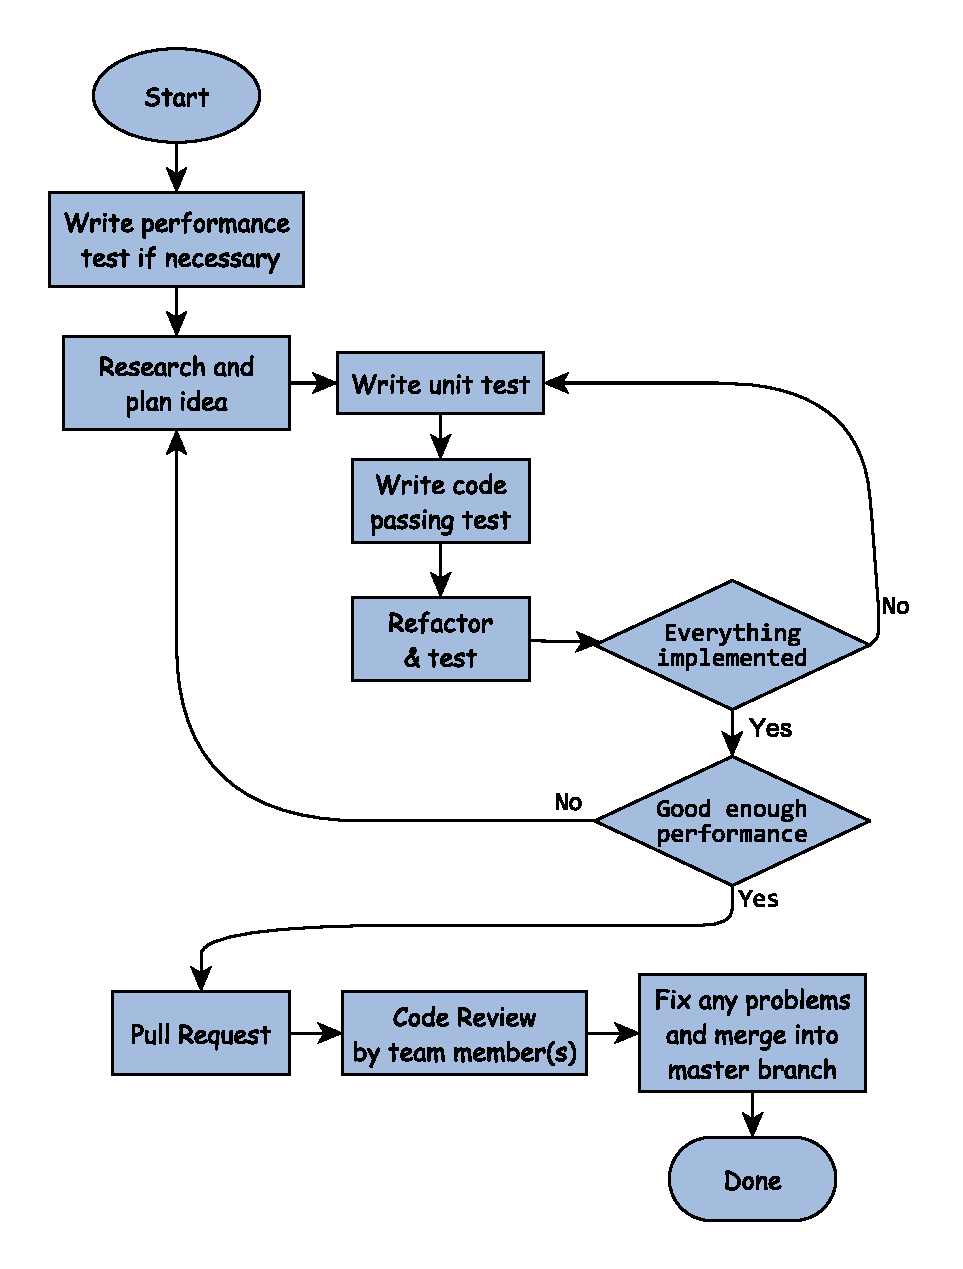
\includegraphics[width=120mm]{images/sprint_item_development.eps}
	\caption{\textit{caption...}}
	\label{fig:sprint_development_cycle}
\end{figure}\\
Text here


\newpage
\section{Initial Backlog}
\label{sec:initial_backlog}

\subsection{Sprint planning}

The sprints are, when possible, two weeks long and specified in \ref{sprintdate}. Sprint 2 is shorter due to the exam period and sprint 5 is shorter due to the project deadline.

\label{sprintdate}
\begin{center}
	\begin{Large}
	\begin{tabular}{|c|c|c|c|}
		\hline
		\large{\textbf{Sprint number}} & \large{\textbf{Start}} & \large{\textbf{Finish}} & \large{\textbf{Comment}} \\
		\hline
		\large{0} & \large{2013-09-16} & \large{2013-09-30} & \large{} \\
		\hline
		\large{1} & \large{2013-09-30} & \large{2013-10-14} & \large{} \\
		\hline
		\large{2} & \large{2013-10-14} & \large{2013-10-18} & \large{Margin time} \\
		\hline
		\large{-} & \large{2013-10-21} & \large{2013-11-01} & \large{Exam period} \\
		\hline
		\large{3} & \large{2013-11-04} & \large{2013-11-18} & \large{} \\
		\hline
		\large{4} & \large{2013-11-18} & \large{2013-12-02} & \large{} \\
		\hline	
		\large{5} & \large{2013-12-02} & \large{2013-12-12} & \large{Deadline 2013-12-13} \\
		\hline	
	\end{tabular}
	\end{Large}
\end{center}
\vspace{0.5cm}
The following tables lists backlog items and their priotiries for each sprint. \\

\label{sprint0}
\begin{center}
	\begin{Large}
	\begin{tabular}{|p{10.5cm}|c|c|}
		\hline
		\multicolumn{3}{|c|}{\textbf{Sprint 0}} \\
		\hline
		\large{\textbf{Item}} & \large{\textbf{Priority}} & \large{\textbf{Req. No.}} \\
		\hline
		\large{Requirement specification finalized} & \large{1} & - \\
		\hline
		\large{Project plan finalized} & \large{1} & 7.1 \\
		\hline
		\large{A running test system} & \large{1} & - \\
		\hline
		\large{Initial test data gathered} & \large{1} & 5.10 \\
		\hline
		\large{Initial test data labeled} & \large{2} & 5.10 \\
		\hline
		\large{Build system deployed} & \large{1} & - \\
		\hline	
		\large{A code standard} & \large{1} & - \\
		\hline	
		\large{An initial code skeleton} & \large{1} & - \\
		\hline	
		\large{DOxygen deployed} & \large{2} & - \\
		\hline		
	\end{tabular}
	\end{Large}
\end{center}



\label{sprint1}
\begin{center}
	\begin{Large}
	\begin{tabular}{|p{10.5cm}|c|c|}
		\hline
		\multicolumn{3}{|c|}{\textbf{Sprint 1}} \\
		\hline
		\large{\textbf{Sprint item}} & \large{\textbf{Priority}} & \large{\textbf{Req. No.}} \\
		\hline
		\large{Stream video from camera to screen} & \large{1} & - \\
		\hline
		\large{Segmentation of Background-Forground} & \large{1} & - \\
		\hline
		\large{Forground labeling} & \large{1} & - \\
		\hline
		\large{Basic tracking of objects} & \large{1} & - \\
		\hline
		\large{Simple self callibration (illumination)} & \large{2} & 5.8 6.3 \\
		\hline
		\large{Estimate flow of people} & \large{1} & 5.1 5.2 5.3 \\
		\hline
		\large{Real time visualization of intermediate steps of the program} & \large{1} & - \\
		\hline
	\end{tabular}
	\end{Large}
\end{center}



\label{sprint2}
\begin{center}
	\begin{Large}
	\begin{tabular}{|p{10.5cm}|c|c|}
		\hline
		\multicolumn{3}{|c|}{\textbf{Sprint 2}} \\
		\hline
		\large{\textbf{Sprint item}} & \large{\textbf{Priority}} & \large{\textbf{Req. No.}} \\
		\hline
		\large{Basic queue identification} & \large{1} & 5.4 \\
		\hline
		\large{Stream video from more than one camera} & \large{1} & - \\
		\hline
	\end{tabular}
	\end{Large}
\end{center}



\label{sprint3}
\begin{center}
	\begin{Large}
	\begin{tabular}{|p{10.5cm}|c|c|}
		\hline
		\multicolumn{3}{|c|}{\textbf{Sprint 3}} \\
		\hline
		\large{\textbf{Sprint item}} & \large{\textbf{Priority}} & \large{\textbf{Req. No.}} \\
		\hline
		\large{Improved tracking of objects (Occlusions etc.)} & \large{1} & - \\
		\hline	
		\large{Identify/unique persons} & \large{1} & - \\
		\hline	
		\large{Group cameras according to room} & \large{1} & - \\
		\hline
		\large{Multiple-camera people-identification} & \large{2} & - \\
		\hline
		\large{Callibration of multiple cameras} & \large{2} & - \\
		\hline
		\large{Estimate number of people in queue} & \large{2} & 5.7 \\
		\hline
		\large{Estimate queue time} & \large{2} & 5.7 \\
		\hline
	\end{tabular}
	\end{Large}
\end{center}



\label{sprint4}
\begin{center}
	\begin{Large}
	\begin{tabular}{|p{10.5cm}|c|c|}
		\hline
		\multicolumn{3}{|c|}{\textbf{Sprint 4}} \\
		\hline
		\large{\textbf{Sprint item}} & \large{\textbf{Priority}} & \large{\textbf{Req. No.}} \\
		\hline
		\large{Improved queue identification} & \large{3} & 5.5 5.6 \\
		\hline
		\large{A administration program} & \large{1} & 6.2 6.4 \\
		\hline
		\large{A installer GUI} & \large{1} & 6.1 \\
		\hline
		\large{The system is tested in realistic conditions (changing illumination, lights turning on/off..)} & \large{1} & 5.9 \\
		\hline
	\end{tabular}
	\end{Large}
\end{center}



\label{sprint5}
\begin{center}
	\begin{Large}
	\begin{tabular}{|p{10.5cm}|c|c|}
		\hline
		\multicolumn{3}{|c|}{\textbf{Sprint 5}} \\
		\hline
		\large{\textbf{Sprint item}} & \large{\textbf{Priority}} & \large{\textbf{Req. No.}} \\
		\hline
		\large{A project report} & \large{1} & 7.2 \\
		\hline
		\large{A user manual} & \large{1} & 7.3 \\
		\hline
		\large{A project webpage} & \large{1} & 6.5 \\
		\hline
	\end{tabular}
	\end{Large}
\end{center}



%
% Bibliography
%

% Force a blank page so the bibliography starts on a new page.
% Comment out if not necessary
%\newpage
\thispagestyle{fancy}
\mbox{}
\newpage
\begin{thebibliography}{9}
\addcontentsline{toc}{section}{References} % Add an entry for this in the table of contents

\bibitem{Gardel}
	Gardel, A., Bravo, I., Jimenez, P., Lazaro, J.L. \& Torquemada, A.\\
	``\textit{Statistical Background Models with Shadow Detection for Video Based Tracking},''\\ Intelligent Signal Processing, 2007. WISP 2007. IEEE International Symposium on?? Page: 1-6.
	
\bibitem{Zivkovic}
	Zivkovic, Z. \& Heijden, F.\\
	``\textit{Efficient Adaptive Density Estimation per Image Pixel for the Task of Background Subtraction},''\\
	Pattern recognition letters, Vol. 27, No. 7. (2006), pp. 773-780.

\vspace{2cm}
\LARGE{\textbf{EXAMPLE REFERENCES ONLY, REMOVE BEFORE HANDING IN}}
\normalsize
\bibitem{CVBook}
	Sonka, M., Hlavac, V. \& Boyle, R. 
	\emph{Image Processing, Analysis, and Machine Vision}.\\
	Toronto: Thompson Learning,
	cop. 2008, 3rd ed.,
	ISBN 0495244384.
	
\bibitem{Wood}
	Wood, J. (2007)
	``\textit{Statistical Background Models with Shadow Detection for Video Based Tracking},''\\
	Master thesis, Linköping University, Department of Electrical Engineering.	

\bibitem{DSPBook}
	Gustafsson, F., Ljung, L. \& Millnert, M.
	\emph{Signal Processing}.\\
	Studentlitteratur, Lund, Sweden,
	2011, 1st ed.,
	ISBN 978--91--44--05835--1.

\bibitem{MOTA}
	Bernardin, K. \& Stiefelhagen, R (2008)\\
	``\textit{Evaluating Multiple Object Tracking Performance: The CLEAR MOT Metrics},''\\
	Interactive Systems Lab, Institut für Theoretische Informatik,\\
	Universität Karlsruhe, 76131 Karlsruhe, Germany

\bibitem{CAVIAR}
	``\textit{CAVIAR: Context Aware Vision using Image-based Active Recognition},''\\
	EC Funded CAVIAR project/IST 2001 37540\\
	http://homepages.inf.ed.ac.uk/rbf/CAVIAR/
	

%\bibitem{somePaper}
%	Q. Lastname,
%	``Some article title,''
%	\emph{Some scientific journal},
%	vol.~1337, no.~1337,
%	pp.~666--1337,
%	month.~1337.

\end{thebibliography}



\end{document}
